% !TEX root = report.tex
\noindent\begin{minipage}[t]{0.56\textwidth}\vspace{0pt}
\textbf{Current state:} \texttt{wargame\_gui.py} runs the model of \S3 as a \textbf{GUI} (Fig.~\ref{fig:gui}: pick
each side's plan, Blue's design and the weather, then step through turns or run many games; a Help button explains
the map), as \textbf{batch} runs, or as a turn-by-turn \textbf{trace}. \texttt{experiments.py all} regenerates
every number in \S4; instructions are in \texttt{README.md}.

\smallskip\noindent \textbf{How the code reflects the model:} \texttt{Game.step} is the timeline of Fig.~\ref{fig:net} with
\eqref{eq:control}--\eqref{eq:payoff}; \texttt{MIPBRPolicy} solves the MIP of \S\ref{sec:mip} each period;
\texttt{MetaGame} builds $\Gamma$ and runs IESDS, NE enumeration and both LPs.

\smallskip\noindent 
\textbf{Still to build:} Learning agents, an attacker that reacts to Blue, Bayesian beliefs and multi-period
policies (\S6).
\end{minipage}\hfill
\begin{minipage}[t]{0.41\textwidth}\vspace{0pt}\centering
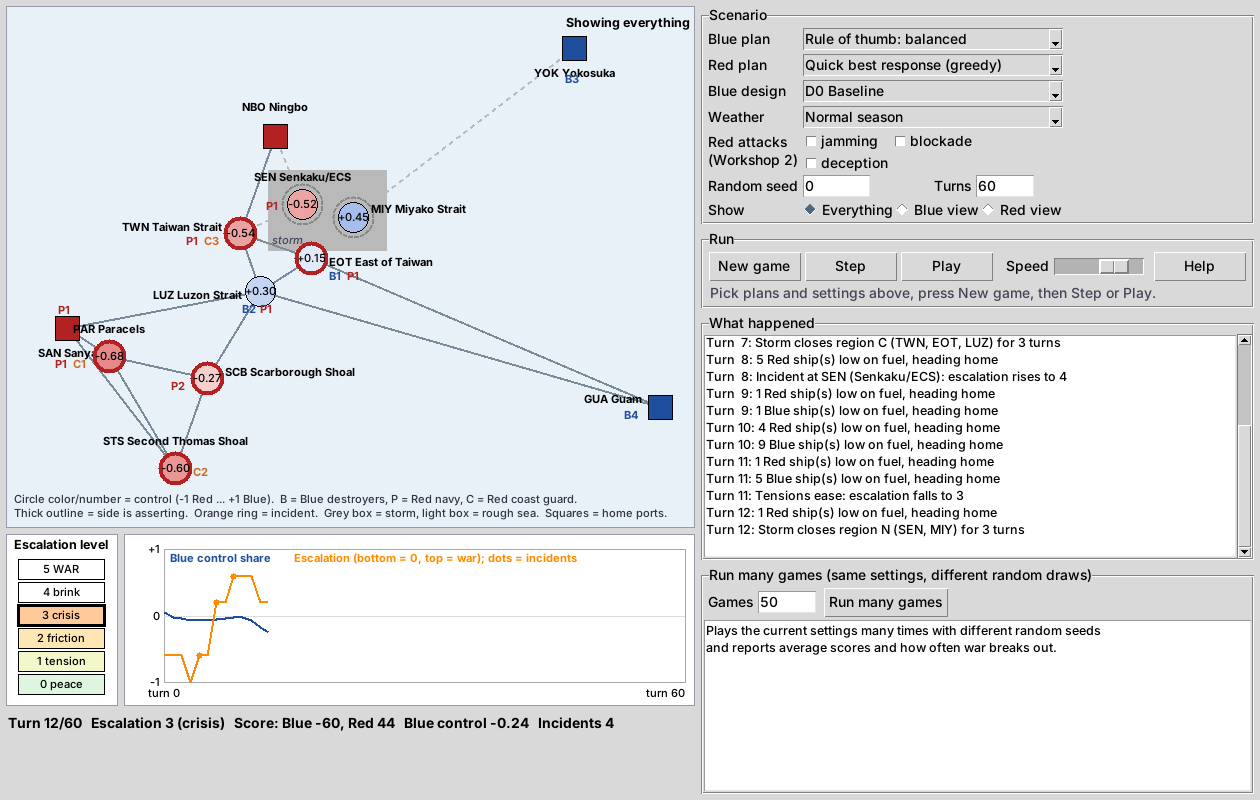
\includegraphics[width=\textwidth]{figures/gui_screenshot.png}
\captionof{figure}{The GUI after 12 turns (storm in the North).}\label{fig:gui}
\end{minipage}
